\documentclass[main.tex]{subfiles}

\begin{document}

	\begingroup

	\renewcommand{\cleardoublepage}{}

	\renewcommand{\clearpage}{}

	\chapter{Clean Up Task Overview}
	\label{cleanup-sequence}

		\chapterauthor{~\\Torge Olliges,\\ Jan Schimpf, Jeremias Thun}
		
		\section{Goal}
		The goal of the Clean Up task is like the name indicates to clean a room. In the RoboCup several objects get distributed throughout the room. The objects can be placed on the floor, tables, or other furniture. Each of these objects is visible and not hidden behind something. The task of the HSR is now to find these objects and place them into a designated basket. There exist multiple target positions and the HSR has to decide by itself the correct one based on the object. Like the Storing Grocery task the time limit is 5 minutes.

	  	\section{Tasks}
	  	The figure \ref{clean_up_seq_01} shows the procedure of Clean Up. The following subsections explain the execution and procedure in detail and give insights into the decisions made resulting in the exact plan depicted below. As well as for the Grocery Storing task, there will be a description of the most important sequences below.

	  	\begin{figure}	
	  		\centering
	  		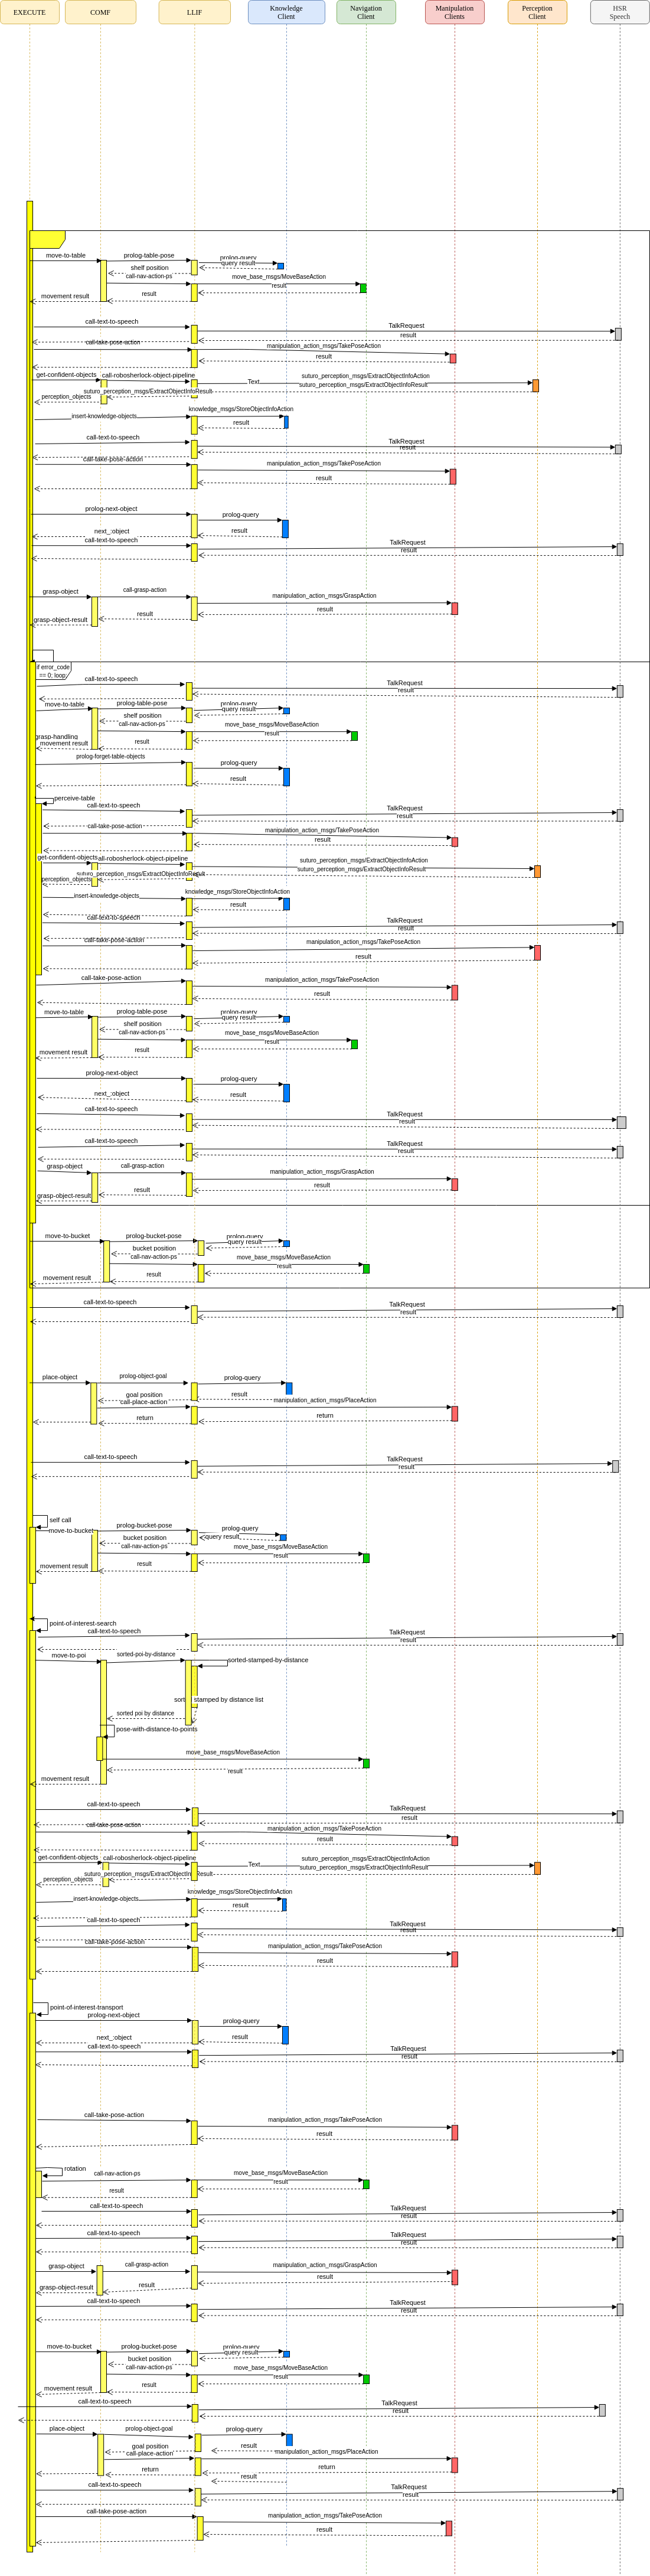
\includegraphics[width=0.85\textwidth]{pictures/diagramms/cleanup-sequence.png}
	  		\caption{Sequence diagram of the complete run of the clean up task \textit{(explanations below)}}
	  		\label{clean_up_seq_01}
	  	\end{figure}
	  	% TODO: Entfernen - hier bitte aus dem sequenz diagramm einen einzelnen task als subsection z.b. schritt: tür öffnen, dafür mussten perception dies tun manipulation das tun etc.
	  	
	\subsection{Setup}
	\begin{knowledge}	
	First the interface to Knowledge is called make the basket a \textit{target} surface and the floor and the table \textit{source} surfaces, since objects are picked up from both.
	\end{knowledge}
	
	% Manipulation: take pose action
	\begin{manipulation}
	Just as described in the task Grocery Storing, Manipulation needs to set the robot to the default pose.
	\end{manipulation}

	\subsection{Scan table sequence}
	
	% Knowledge: get table-poses
	\begin{knowledge}
	The Clean Up task starts by looking into the objects on the table(s), so Knowledge is needed to provide the position of the nearest table.
	\end{knowledge}
	
	% Navigation: moveBaseAction
	\begin{navigation}
	To perceive the table, the robot is again turned $90^\circ$ to the table. Allowing it to look over its shoulder having a clear view of the table.
	\end{navigation}
	
	% NLP
	\begin{nlp}
	Before the robot can start to perceive, the user will be informed by the computer voice, that the robot is now perceiving the table.
	\end{nlp}
	
	% Manipuilation: TakePoseAction
	\begin{manipulation}
	With the robot standing at the right spot, it is the task of Manipulation to get it into a position where it can perceive the table.
   \end{manipulation} 
	
	% Perception: Percieve and return data
	\begin{perception}
	In this position the table will be scanned and Perception again generates all necessary information about the objects standing on the table.
	\end{perception}
	
	% Knowledge: Store Data
	\begin{knowledge}
	As in the similar sequences in Grocery Storing, Knowledge stores the perceived data in the Knowledge base.
	\end{knowledge}
	% NLP: Talk Request
	
	% Manipulation: Take pose
	\begin{manipulation}
	To prepare for grasping, the robot is put back in its default position.
	\end{manipulation}
	
	% 2x NLP: Talk
	
	
	% Navigation: MoveBaseAction
	\begin{navigation}
	Also, the robot needs to be turned back from the perceiving pose by $90^\circ$ so it looks straight at the table and can grasp an object.
	\end{navigation}
	
	\subsection{Grasp sequence}\label{clean_up_grasp_seq}
	
	%prolog-next-object
	\begin{knowledge}
	Knowledge first decides which object to grasp first, which works the same way as in Grocery Storing and is purely based on the distance to the robot.
	\end{knowledge}
	
	%NLP Grasping object
	\begin{nlp}
	The computer voice of the robot is now informing everyone that the robot will now grasp an object. Right after that it also says which object the robot will grasp based on the object id.
	\end{nlp}
	
	%grasp-object
	\begin{manipulation}
	The object id is used to query the Knowledge base for the dimensions of the object and the pose of the object. The results are then used to call the manipulation grasp server to grasp the object. Manipulation then gets the task to grasp the given object.
	\end{manipulation}
	 %Knowledge: prolog dimensions
	 %Knowledge: prolog pose
	 \begin{knowledge}
	 Knowledge again realizes that the gripper now carries an object and attaches that object to the gripper in the Knowledge base.
	 \end{knowledge}
	 
	%NLP succesfully grasped
	\begin{nlp}
	Grasping the object is completed by the robot saying that it has successfully grasped the object.
	\end{nlp}
    
	\subsection{Place sequence}
	%Navigation: moveBaseAction
	\begin{navigation}
	The robot moves to the designated location in this case the bucket.
	The coordinates for the navigation call are queried from the Knowledge base and adjusted so the robot looks at the bucket and can place the object inside it. 
	\end{navigation}
	
	%NLP placing the object
	\begin{nlp}
	The robot then informs everyone that it is now placing the object
	\end{nlp}

	\begin{knowledge}
	To correctly place the object in the bucket, Knowledge just calculates some offsets to the middle of the bucket and completely ignores, whether there already are some objects in it or not. To Knowledge, the bucket surface is a black hole where an infinite number of objects can be placed in the same spot.
	\end{knowledge}

	%place-object
	\begin{manipulation}
	 Manipulation then gets the task to place the previously grasped object in the given destination. To do that the Place Action Server has to calculate the correct orientations to place from the right direction and do collision avoidance with all other objects which is done by using \textit{Giskard}.
	 \end{manipulation}
	 %Knowledge: prolog dimensions
	 %Knowledge: prolog goal
	 
	%NLP placed the object
	\begin{nlp}
	This is where the robot informs everyone, that the object has been successfully placed.
	\end{nlp}

	%Manipulation: Take pose
	\begin{manipulation}
	To start again, the robot is put in the default pose again.
	\end{manipulation}
	
	\begin{planning}
	This whole part restarts by asking Knowledge for the next object to grasp until there are no objects left on the table. After that, there is a second loop where the robot looks for points of interest and stops if there are not points of interest left.
	\end{planning}
	
	\subsection{Point of interest search sequence}
	\begin{navigation}
	The object finder node publishes based on the data of the laser scanner in the foot of the robot a list of poses that may be an object. This list will from now on be called points of interest.
	\end{navigation}
	
    %NLP found an point of interest to search
    \begin{nlp}
    The speech client starts this sequence by telling everyone that the robot has found a point of interest to search for objects.
    \end{nlp}
    
    %move-to-poi
    \begin{planning}
    The first pose of the points of interest is taken. A target position is calculated that enables the HSR to perceive the position.
    This target pose is then sent to navigation and executed.
   \end{planning}
   
    %call-take-pose-action
    \begin{manipulation}
    The HSR is then brought into the perceive pose for the floor.
    \end{manipulation}
    
    %NLP perceiving the postition
    \begin{nlp}
    When the robot is ready to perceive, it says so via its speech client.
    \end{nlp}
      
    %call-robosherlock-object-pipeline
    \begin{perception}
	Looking at the floor at this point of interest, the robot makes a picture that Perception can again use to find the objects that are hopefully standing there. Once there are objects found, the data will be published.
	\end{perception}
    
    %Knowledge:insert-knowledge-objects
	\begin{knowledge}
	These perceived object data will find their way to Knowledge where they are looked into and stored as they make any sense.
	\end{knowledge}
    
	\begin{planning}
	Now the objects that were found are one by one grasped and placed in the basket in the same way, the objects standing on the table were handled.
	
	This continues until there are no known objects and no points of interest left anymore.
	\end{planning}
    
	\section{Conclusion}
	The Clean Up task was still incomplete for the simulated RoboCup at the end of the second milestone and wasn't executed due to having various problems getting the robot to run in the challenge room, but was in an executable and working state for the third milestone demo and completed the demo run. During this run, it showed that the tasks grasping the objects of the table or from the floor, transporting the objects and placing them in the basket were achieved in the simulation.\\
	Even with the run being completed the plan has similar problems to the Grocery Storing task with the magnet sensors and there are still potential issues as the way items on the floor are currently searched for involves the laser scanner so items that are too small to be picked up by the laser scanner won't be found by the robot.\\
	Overall the Clean Up task can be considered as a success as all the necessary tasks that are part of the Clean Up challenge can be completed. 
	
	\endgroup

\end{document}

